% Preamble templated from Mihir-Divyansh/Course-Setup
%iffalse
\let\negmedspace\undefined
\let\negthickspace\undefined
\documentclass[journal,12pt,onecolumn]{IEEEtran}
\usepackage{cite}
\usepackage{amsmath,amssymb,amsfonts,amsthm}
\usepackage{algorithmic}
\usepackage{graphicx}
\usepackage{textcomp}
\usepackage{xcolor}
\usepackage{txfonts}
\usepackage{listings}
\usepackage{enumitem}
\usepackage{mathtools}
\usepackage{gensymb}
\usepackage{comment}
\usepackage[breaklinks=true]{hyperref}
\usepackage{tkz-euclide}
\usepackage{listings}
\usepackage{gvv}
%\def\inputGnumericTable{}
\usepackage[latin1]{inputenc}
\usepackage{color}
\usepackage{array}
\usepackage{longtable}
\usepackage{calc}
\usepackage{multirow}
\usepackage{hhline}
\usepackage{ifthen}
\usepackage{lscape}
\usepackage{tabularx}
\usepackage{array}
\usepackage{float}
\usepackage{caption}
\usepackage{multicol}

\newtheorem{theorem}{Theorem}[section]
\newtheorem{problem}{Problem}
\newtheorem{proposition}{Proposition}[section]
\newtheorem{lemma}{Lemma}[section]
\newtheorem{corollary}[theorem]{Corollary}
\newtheorem{example}{Example}[section]
\newtheorem{definition}[problem]{Definition}
\newcommand{\BEQA}{\begin{eqnarray}}
\newcommand{\EEQA}{\end{eqnarray}}
%\newcommand{\define}{\stackrel{\triangle}{=}}
\theoremstyle{remark}
%\newtheorem{rem}{Remark}

% Marks the beginning of the document
\begin{document}
\bibliographystyle{IEEEtran}
\vspace{3cm}

\title{Assignment 10: 5.2.57}
\author{EE25BTECH11055 - Subhodeep Chakraborty}
\maketitle
\hrulefill
\bigskip

\renewcommand{\thefigure}{\theenumi}
\renewcommand{\thetable}{\theenumi}

\textbf{Question:}\par
Solve the following system of linear equations.
\begin{align*}
 2x+y+z&=1\\
 x-2y-z&=\frac{3}{2}\\
 3y-5z&=9
\end{align*}
\par
\textbf{Solution:}\par

Given:
\begin{align}
 \vec{n_1}^\top\vec{x}&=c_1 &\vec{n_1} = \myvec{2\\1\\1} c_1 = 1\\
 \vec{n_2}^\top\vec{x}&=c_2 &\vec{n_2} = \myvec{1\\-2\\-1} c_2 = 3/2\\
 \vec{n_3}^\top\vec{x}&=c_3 &\vec{n_3} = \myvec{0 \\3 \\ -5} c_3 = 9
\end{align}

Thus
\begin{align}
  \myvec{\vec{n_1} & \vec{n_2} & \vec{n_3}}^\top\vec{x} = \myvec{c_1\\c_2\\c_3}
\end{align}
On forming augmented matrix and applying Gaussian elimination, we can solve for $\vec{x}$
\begin{align}
 \implies \augvec{3}{1}{2&1&1&1\\1&-2&-1&3/2\\0&3&-5&9} \xleftrightarrow[]{R_2=2R_2-R_1} \\
 \augvec{3}{1}{2&1&1&1\\0&-5&-3&2\\0&3&-5&9} \xleftrightarrow[]{R_3=5R_3+3R_2}
 \augvec{3}{1}{2&1&1&1\\0&-5&-3&2\\0&0&-34&51} \\
 \xleftrightarrow[]{R_3=-R_3/34; R_2=R_2+3R_3}
 \augvec{3}{1}{2&1&1&1\\0&-5&0&-5/2\\0&0&1&-3/2} \xleftrightarrow[]{R_2=-R_2/5; R_1=R_1-R_2-R_3}
 \augvec{3}{1}{2&0&0&2\\0&1&0&1/2\\0&0&1&-3/2} \\
 \xleftrightarrow[]{R_1=R_1/2}
 \augvec{3}{1}{1&0&0&1\\0&1&0&1/2\\0&0&1&-3/2}
\end{align}
So we have:
\begin{align}
 \vec{x}=\myvec{x\\y\\z}=\myvec{1\\1/2\\-3/2}
\end{align}
\begin{figure}[H]
    \centering
    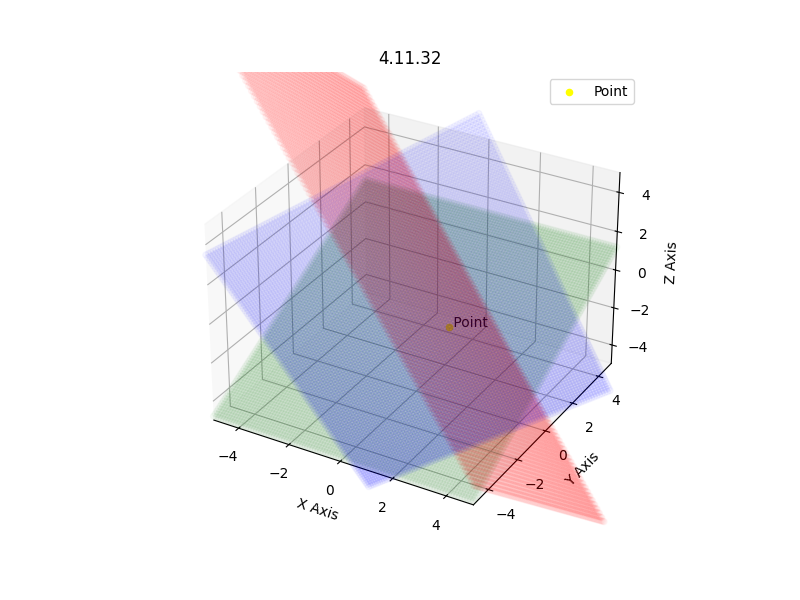
\includegraphics{figs/plot.png}
    \caption*{}
    \label{fig:plot}
\end{figure}
\end{document}
